\documentclass[11pt,a4paper]{article}
\usepackage[margin=23mm,headheight=15pt]{geometry}
\usepackage{fontspec}
\setmainfont{Times New Roman}
\setsansfont{Arial}
\usepackage{amsmath,amssymb,graphicx,booktabs,array,tabularx,longtable,caption,xcolor,fancyhdr,enumitem,placeins}
\usepackage[numbers,sort&compress]{natbib}
\usepackage[colorlinks=true,linkcolor=teal!55!black,citecolor=teal!55!black,urlcolor=teal!55!black]{hyperref}
\definecolor{navy}{HTML}{193447}
\definecolor{pale}{HTML}{EDF4F5}
\usepackage{titlesec}
\titleformat{\section}{\large\sffamily\bfseries\color{navy}}{}{0em}{}
\setlength{\parindent}{0pt}
\setlength{\parskip}{6pt}
\raggedbottom
\setlength{\emergencystretch}{3em}
\widowpenalty=10000\clubpenalty=10000
\renewcommand{\topfraction}{.95}\renewcommand{\bottomfraction}{.85}\renewcommand{\textfraction}{.05}\renewcommand{\floatpagefraction}{.75}
\renewcommand{\arraystretch}{1.16}
\captionsetup{font=small,labelfont=bf,justification=raggedright,singlelinecheck=false}
\pagestyle{fancy}\fancyhf{}\fancyhead[L]{\small\sffamily EVIDENCE TO EXPERIMENT}\fancyhead[R]{\small\sffamily 17 November 2026}\fancyfoot[C]{\thepage}
\renewcommand{\headrulewidth}{0.3pt}
\graphicspath{{figures/}}
\newcounter{boxnum}
\newcommand{\boxlabel}{Box}
\usepackage{xeCJK}
\setCJKmainfont{SimSun}[BoldFont=SimHei,ItalicFont=KaiTi]
\setCJKsansfont{Microsoft YaHei}
\renewcommand{\figurename}{图}\renewcommand{\tablename}{表}\renewcommand{\refname}{参考文献}\renewcommand{\boxlabel}{框}
\usepackage[mathlines]{lineno}
\setlength{\linenumbersep}{8pt}
\renewcommand\linenumberfont{\normalfont\tiny\sffamily}
\begin{document}\runninglinenumbers
{\small\sffamily\color{navy} PERSPECTIVE | 证据综合}\par\medskip
{\LARGE\bfseries\raggedright 运动学习中的共享与分离：整合迁移、分离与误差归因证据\par}\bigskip
{\normalsize JiaHao Wu、曾龙（Long Zeng）\par}
{\small 清华大学深圳国际研究生院，中国深圳\par}\medskip
\hypersetup{pdfauthor={JiaHao Wu; Long Zeng}}
{\small 通讯作者：曾龙（Long Zeng），\href{mailto:zenglong@sz.tsinghua.edu.cn}{zenglong@sz.tsinghua.edu.cn}\par}\medskip
\section{摘要}
相似的适应动作可以由不同学习机制产生。本文沿输入、输出和时间尺度整合迁移、分离、误差归因及感觉特异性证据。具体案例展示时间混合与感知测量如何影响机制推断。公开数据重分析说明跨研究预测及其边界：增加时间成分改善补偿预测，共同与分别模型的排序随分析设定变化。证据地图将竞争解释连接到针对性测量、对照和预测。该框架指导运动神经科学中的实验选择，并为评估任务表现相似的具身控制器提供前瞻性方法。

\section{从力场实验提出问题}
设想一个人在侧向力场中学习到达目标。手的轨迹逐渐变直；随后施加的机械脉冲揭示纠错响应发生变化，通道试次则显示预期性补偿。两类测量共同确立了训练影响多个控制成分。科学问题在于这些成分的联系产生于何处：共同的动力学表征、学习过程间的通信、共同误差信号，或已有知识在当前任务中的表达。力场与手臂动力学改变实验能够在同一装置内测量扰动、力和肌肉活动，为回答这一问题提供直接条件。\cite{wagner2008,maeda2018,maeda2020}

文献也记录了选择性变化。力场暴露的时间一致性对前馈与反馈结构学习产生不同影响；镜像反转学习依赖在线动作后果是否可见；视觉误差对即时纠错的影响可以强于对后续适应的影响。这些结果共同约束理论：解释必须同时覆盖迁移与选择性变化，并说明各自的发生条件。\cite{yousif2012,kasuga2015,hoffmann2023}

本文的组织观点是，共享需要说明\emph{共享什么、连接哪些输出，以及发生在哪个时间区间}。我们将感觉通道、控制输出和时间尺度放在独立轴上，再用误差表征、更新、保持和表达的过程连接它们。这一组织方式导出具体比较：输入层争议需要经过检验的观测模型，表达层争议需要交叉情境测试，教学信号争议需要配对的时间响应。补充证据图谱E01--E29提供这些选择的逐实验依据。


\begin{figure}[!htbp]\centering
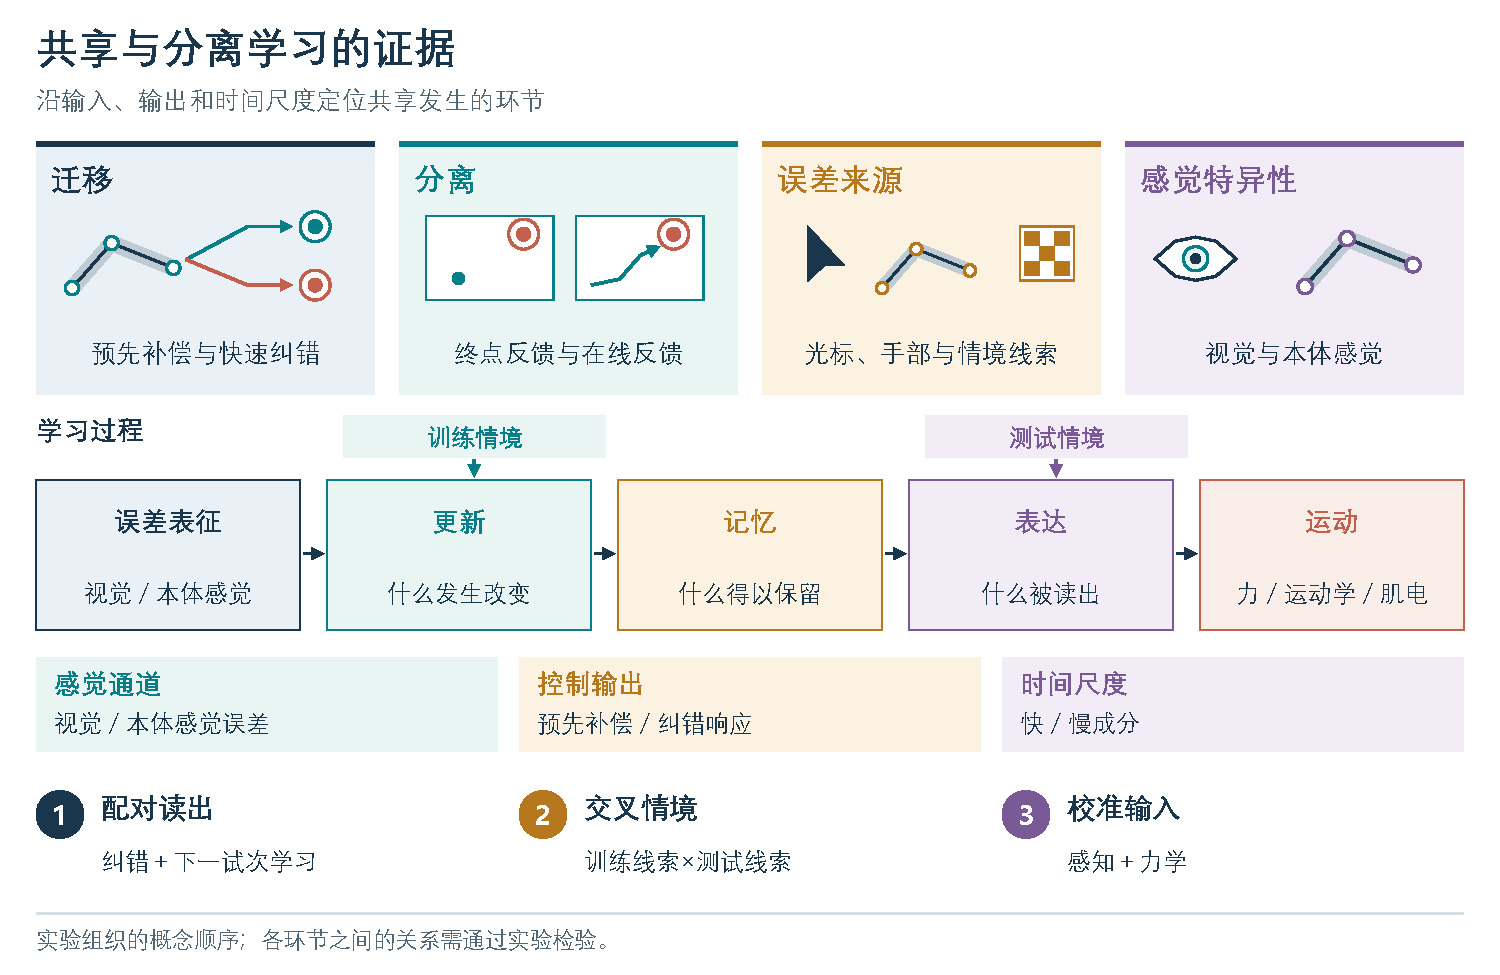
\includegraphics[width=\textwidth]{figure1_zh.pdf}
\caption{证据线索与拟议整合。四类观察约束不同学习环节，以及感觉通道、控制输出和时间尺度三个独立维度。流程组织实验比较。文字、图形与连线由PowerPoint原生对象组成，表示待检验的概念关系。}
\end{figure}
\section{证据地图的构建}
证据地图采用目的性批判综合：纳入能够连接至少两项相关测量、选择性操纵学习条件或提供竞争实现的研究。更新版进一步检索目标误差、不确定性、注意及感知误差研究，检查它们对核心主张的挑战。八张结论卡记录支持、针对当前或更强主张的反证、范围及由此形成的实验选择；反证审计详见图谱和检索记录。核心领域为人类上肢适应，来源推断与循环网络计算研究用于明确竞争解释。每个条目记录操纵、测量、观察结果、支持的推断、残余解释与拟议判别测试，并给出原文实验、图或结果节定位。原始发现与本文提出的测试分别存放。检索及来源核查更新至2026年11月17日；2026年的eLife条目标明为已评审预印本第1版。\cite{makino2026}

综合单元是具有明确定义读出的实验对比。50--100 ms肌肉响应、251--350 ms视觉诱发力及下一试次后效均保留各自的时间定义与测量含义。推断强度按原研究的具体对照判断。例如，Cluff和Scott通过探针目标控制背景激活，使其证据比两个不受约束输出之间的相关更有信息量。图谱同时保留这些设计优势与残余解释。各类异质结果按实验中的因果作用比较，形成可审计的论证链。\cite{cluff2013,maeda2018,kasuga2015}

\section{迁移确立跨输出利用已学习动力学}
Wagner和Smith发现，纠错响应能够利用已学到的力场动力学（E01）。Maeda及同事直接改变手臂动力学：肩关节固定减少了自主肘关节运动所需的肩部指令，这种学习迁移至肩关节释放时测得的长潜伏期响应（E02）；随后，训练扰动响应又在反方向迁移至自主到达（E03）。Cluff和Scott在控制探针目标处肌肉激活的同时，测得具有负载特异性的长潜伏期响应变化（E08）。这些实验共同支持：一种控制条件下获得的经验，会改变另一条件对肢体动力学的响应。\cite{wagner2008,maeda2018,maeda2020,cluff2013}

这一结论约束机制解释。共享动力学估计可以为两个输出提供更新后的预测；不同适应通路可以传递更新，或接收共同教学信号；循环控制器则可将动力学相关响应嵌入策略。反馈训练的循环实现已复现多项行为与神经学习特征，为显式预测器架构提供了具体竞争者（E21）。因此，关键比较应在匹配正常行为后，检验跨输出、跨干预的联合预测。\cite{feulner2025}

迁移也依赖测试条件。线索可以选择已存储记忆，或改变其读出增益。COIN框架及诱发恢复实验展示了情境推断如何影响记忆表达与更新（E19）。训练线索乘测试线索的二乘二交叉设计可以直接揭示这种歧义：首次无误差探针上的测试线索效应识别表达贡献；在共同测试线索下保留的训练线索效应，则推动对获得、保持与持续输入重校准的比较。由此，不同观察可归入迁移过程的不同阶段。\cite{coin2021}

\section{分离揭示耦合的发生条件}
Yousif和Diedrichsen在匹配各类暴露试次数量的条件下操纵时间一致性。一致经验同时改变前馈与反馈测量中的结构学习；不一致经验改变反馈结构，却未引起相应前馈结构变化（E04）。这一结果将扰动历史纳入机制解释：若模型对两个读出施加相同且无条件的更新，就必须解释时间组织为何改变二者关系。不同时间尺度、情境选择和选择性更新提供了明确的竞争解释。\cite{yousif2012}

Kasuga及同事操纵镜像反转到达训练中的在线视觉后果（E05）。终点反馈支持更好的前馈表现，连续反馈使不适当纠错响应更明显地衰减。该研究测量的是较晚时间窗的视觉诱发力，与前述机械长潜伏期响应有不同时间定义；镜像反转还改变了所需策略映射。由此形成有价值的比较：动力学改变下的知识迁移与新反馈映射的获得，对经验提出不同要求。比较需要匹配暴露、训练时长与基线表现。\cite{kasuga2015}

时间尺度还提供了另一层区分。Crevecoeur及同事在不可预期动力学下观察到进行中运动的力场特异调整（E11）。这种试次内适应可以在持续的下一试次改变形成之前改善终点表现。因此，配对设计应同时测量当前纠错的变化及其在后续探针中的保留，再用多延迟测试区分瞬时控制调整与较慢保持过程。\cite{crevecoeur2020}

\section{误差归因取决于候选原因}
“外部”包含生物学意义不同的原因：可以忽略的显示位移、将再次出现的外力、意外的物体质量，对应不同的有效响应。“内部”也可指随机执行噪声，或肢体动力学的持续变化。Berniker和Kording形式化了这种差别：推断出的身体与世界变化产生不同泛化预测（E13）。Wei和Kording则将非线性误差敏感性与所推断的误差相关性联系起来（E14）。因此，来源、持续性与行为相关性需要分别记录。\cite{berniker2008,wei2009}

Gastrock及同事通过光标跳变或让手可见来揭示视运动旋转（E15）。后效减小；手可见组的主动减被动定位估计接近零，本体感觉重校准保留；对照与手可见组的直接报告差异仍有不确定性。该结果揭示显示失真信息对不同学习成分的选择性影响。手可见性同时改变感觉信息，因而保持可见性一致的纯线索操纵提供下一项有效对比。\cite{external2020}

Kim及同事比较外加旋转与匹配的自身生成运动误差，发现对外加误差的适应更强（E16）。这里的内部类别是运动变异，其因果推断模型估计外部扰动是否发生。结合两项结果，可形成条件化解释：学习取决于证据支持哪一种潜在原因，以及测量哪一个行为成分。“外部归因降低学习”这一预测缺少同时解释两项实验所需的区分。更有判别力的测试应交叉来源可信度与持续性，匹配物理和感知误差，再分别测量感觉与运动后果。\cite{piece2025}

\section{感觉特异学习可以支持共享的控制输出}
Hayashi及同事独立改变视觉与本体感觉误差，包括符号相反的误差条件（E17）。非线性后效与模态相关学习动态支持分别的感觉记忆及交互误差处理解释。这些证据约束学习的输入维度。两个感觉特异状态仍可同时参与预期补偿和纠错控制，因此，视觉与本体感觉记忆分别存在、前馈与反馈控制之间发生迁移，可以在同一架构内成立。\cite{hayashi2020}

Hoffmann及同事将两个维度纳入同一实验（E18）。力扰动中缩放视觉位移，对在线纠错的影响比对后续后效更一致；控制隐藏手的指示消除了视觉对适应的残余影响。任务目标会改变感觉证据与纠错、学习之间的关系。因此，目标乘可靠性的交叉实验应独立校准感知位移，并用固定的已学习参数预测未训练组合。\cite{hoffmann2023}

Izawa和Shadmehr说明了增加感觉后果测量的价值：感觉误差驱动与奖励驱动学习产生不同感觉重映射（E12）。Gastrock及同事通过主动与被动定位进一步展开这一逻辑。这些测量能够揭示到达终点遗漏的输入或预测变化。主动减被动报告本身也是一个测量模型，需要匹配报告要求并评估定位可靠性。\cite{izawa2011,external2020}

\section{时间尺度混合如何解释表面矛盾}
感觉特异学习与跨输出迁移约束学习系统的不同维度。Hayashi等已提出分别的视觉和本体感觉记忆在输出端整合；Smith等确立了快慢适应过程的交互。将这些先例与迁移实验结合，可得到有实验价值的解释：每个输入能够激发多个时间模式，每个输出读取这些模式的不同比例。相应的脉冲响应为
\begin{equation}B_{ij}(k)=\sum_{r=1}^{m}h_{ir}a_r^k u_{rj}.\label{eq:worked}\end{equation}
其中$k$表示无误差保持步数，$a_r$为保持系数，$u_{rj}$表示输入对模式$r$的作用，$h_{ir}$表示该模式对输出$i$的贡献。这一构造解释了不同感觉学习动态如何与向预期运动、纠错响应的迁移并存。本文将比较扩展到多个实验轴；记忆架构的组成来自前人研究。\cite{hayashi2020,smith2006,wagner2008,maeda2020}

固定读出能够产生变化的输出比例。例如，令$H=\left(\begin{smallmatrix}1&0.4\\0.6&1\end{smallmatrix}\right)$、$A=\operatorname{diag}(0.9,0.7)$、$U=\left(\begin{smallmatrix}0.3&0.1\\0.15&0.5\end{smallmatrix}\right)$。在$B(k)=HA^kU$中，第一个输入的输出比例从$k=0$时的1.091变为$k=4$时的1.371；第二个从0.536变为0.713。输入和读出权重始终固定。每个输入激发两种模式，不同衰减率改变其随时间的混合比例。比例恒定要求该输入形成有效一维轨迹，例如只激发一种模式或输出载荷成比例。因此，比例变化排除这一维度限制，并保留固定多模式读出的解释。

判别对象应是完整时间响应。双模式共同动力学模型要求两个输出具有相同特征根，同时允许任意输出幅度；输出特异模型允许不同特征根。在无误差测量中，前者要求所有输入—输出条目满足$B_{ij}(k+2)-(a_1+a_2)B_{ij}(k+1)+a_1a_2B_{ij}(k)=0$。使用多个训练延迟拟合共同递推与输出特异竞争模型，再预测额外延迟及扰动历史。采用独立首次探针、有符号误差、零误差对照及匹配感觉暴露；分母接近零时使用联合响应似然。探针诱发学习须显式进入状态转移。两个延迟对灵活多模式解释的约束较弱。\cite{unlearning2016}

共同时间模式既可由共享状态实现，也可由接收同一误差、分别更新的复制状态实现。随附构造使用输出特异的状态副本复现全部测量响应。因此，行为判别检验的是时间响应家族的限制。物理共享主张需要增加对某个状态或通路作用已被独立测量的干预。显式等价构造据此区分可检验的功能预测与神经实现主张。

\section{具有明确观测量的联合解释}
证据支持三个命题：已学习动力学能够影响多个控制输出；这种耦合依赖训练统计与感觉可用性；感觉、情境及力学过程都能改变所测迁移。本文将其整合为\emph{部分可分过程之间的条件性耦合}。这一综合预测：独立操纵输入、训练情境、测试情境和延迟，将产生具有结构的迁移变化。其经验目标是受控误差到后续所测输出的有效映射。

在指定基线附近的小扰动条件下，可写为
\begin{equation}\Delta\mathbf y_{t+k}=H(q_{\mathrm{test}})A^kU(q_{\mathrm{train}})E(s)\mathbf e_t+\boldsymbol\epsilon.\label{eq:factor}\end{equation}
其中，$\mathbf e_t$为物理视觉和本体感觉误差；$E$在感觉条件$s$下将其映射为有效感觉误差；$U$更新潜在学习状态；$A$描述局部保持；$H$将状态映射为预期补偿及标准反馈探针响应。训练情境与测试情境分别进入模型。该式为实验对比提供局部记账模型；非线性饱和、策略改变与机械输出映射需要相应扩展。因子分解是本文提出的综合表示，其组成现象由E01--E29支撑。

这一表示使四种解释可直接比较。标量门控解释用来源依赖增益乘以固定更新；输入解释改变$E$；表达解释改变$H$；路由解释改变$U$跨感觉输入与控制后果的结构。两个感觉特异潜状态可以在$U$中具有不同列，同时均参与$H$的每一行。由此，感觉特异性与跨输出迁移获得明确的联合实现。

实验在给定条件下辨识的是乘积$B=HA^kUE$。共享潜在更新与同步的分别更新能够产生相同乘积。因此，机制推断需要独立测量因子，并测试竞争分解在其中预测不同乘积的新条件。本文的核心预测是：施加独立验证的观测与时间约束后，联合迁移响应仍随条件变化。支持该预测的证据将确立有效学习的条件性重新分配；进一步定位神经存储与细胞更新机制，需要选择性得到独立验证的干预。

\begin{table}[!htbp]\small\caption{证据支持不同解释层级；编号对应详细图谱。}\label{tab:synthesis}
\begin{tabularx}{\textwidth}{>{\raggedright\arraybackslash}X>{\raggedright\arraybackslash}X>{\raggedright\arraybackslash}X}\toprule
\textbf{证据} & \textbf{已支持推断} & \textbf{整合预测}\\\midrule
迁移（E01--E03、E08） & 动力学知识影响多个输出。 & 交叉训练/测试情境测量跨输出迁移。\\[5pt]
分离（E04--E07、E11） & 耦合依赖暴露与时序。 & 匹配延迟，配对完整纠错与学习波形。\\[5pt]
归因（E13--E16、E19） & 来源与情境影响特定学习/读出成分。 & 交叉来源与持续性，独立校准感知。\\[5pt]
感觉特异性（E12、E17--E18） & 不同感觉输入可产生不同学习后果。 & 同时检验不同输入动态及向两个控制输出的迁移。\\[5pt]
\bottomrule\end{tabularx}\end{table}
\section{反证如何改变实验}
部分分歧在整合后仍然存在，并决定需要哪些追加对照。Tsay等发现，在感觉预测误差存在时，任务误差调节隐式重校准，目标闪烁也会减弱学习（E22）；Oza等将任务误差的收益归于指示敏感的动作选择，并发现可分的隐式重校准（E23）。两项研究围绕自动交互形成具体争议，方案中的目标事件、指示和注意同时不同。共同方案应固定光标误差序列，交叉任务误差与目标闪烁对照，并测量瞄准及即时按指示无反馈后效。交互解释预测残余隐式成分中的任务误差效应；策略叠加解释预测总改善随指示变化而隐式成分稳定。由于瞄准报告本身能够改变策略，各组报告要求须一致。这些预测为共同方案提供竞争检验，现有研究确立了待检验的分歧。\cite{tsay2022,oza2024}

另外两项发现进一步明确对照。Hewitson等观察到对误差大小和方向不敏感的不确定性依赖运动变化（E24）；因此，需要平衡正误差、负误差和零误差，将加性情境变化与误差依赖学习斜率分离。Liddy等发现并行注意任务增强隐式适应，表现依赖反馈使增强持续（E27）；注意对照须记录投入及任务表现，分心系数的方向应由具体方案估计。PReMo与感知预测误差解释还对物理位移所对应的内部误差提出不同主张（E25--E26）。独立定位增加可测约束，留出学习检验所报告感知能否预测目标任务中的教学信号。\cite{uncertain2023,attention2026,premo2022,percept2026}

\section{教学信号的时间形状提供关键检验}
Albert和Shadmehr配对扰动试次肌电与下一通道试次变化，发现缩放且时间提前的对应关系（E06），支持其力场任务中与反馈相关的教学信号。Makino及同事随后在通道内操纵视觉误差时间模式，观察到学习响应仍与运动开始对齐，而持续保持响应可预测学习幅度（E07；已评审预印本）。任务差异本身有信息价值：视觉误差实验检验了原力场对应关系尚未覆盖的时序灵活性。\cite{albert2016,makino2026}

最小追加对比可在同一批参与者中，以配对读出比较两个误差起始时点及一次晚期符号反转，先测试视觉位移，再测试机械上匹配的扰动。在一种起始条件下拟合固定平移复制模型与积分/持续教学模型，统一误差表征与观测噪声，再不重新拟合地预测另一时点及反转条件。复制模型预测学习指令发生相应时间位移；积分教学模型则预测，即使试次内波形变化，保留的误差摘要仍决定学习幅度。在匹配感知误差时改变纠错需求，可继续检验共同上游原因。该设计将分歧集中到波形预测。

\section{感觉校准本身也是测量模型}
定位提供具有自身学习依赖性的额外结果。Gastrock等分别测量主动和被动定位：主动运动将传入信息与运动相关预测结合。这一设计直接支持在报告模型中同时纳入输入和更新相关贡献。在局部差异坐标下，可写为
\begin{align}\delta y&=I+U, &\delta\ell&=C I+L U.\label{eq:calibration}\end{align}
各符号表示物理误差已确定后的条件差异，$C$与$L$为报告载荷。载荷未知时，单项报告无法辨识两种差异；即使载荷已知，$C=L$也使两项测量冗余。设定$C=1,L=0$会把所有报告变化归为输入重校准，从而在观测模型中预置选择性。\cite{external2020,hayashi2020}

其后果可以定量展示。若真实更新变化为$D$、报告载荷$L=1$，则$(\delta y,\delta\ell)=(D,D)$；选择性报告模型用输入变化$I=D$及零更新变化即可精确拟合。新增压力测试在不同交叉载荷下抽取纯机制与混合差异；错误观测模型在测量精确时仍产生这种误判。独立测量$C$和$L$，并使相应观测矩阵具有足够大的奇异值，才可恢复分离。两种载荷趋近时，因子估计的不确定性增长；增加重复无法消除载荷相等时的精确秩亏。

我们下载公开定位档案，重新分析作者按空间插值得到的参与者估计。平均三个报告方向后，对照组主动减被动的适应变化为$-1.54^\circ$（参与者自助法95\%区间$[-2.91,-0.12]$，$n=20$）；手可见组为$-0.02^\circ$（$[-0.86,0.81]$，$n=29$）。直接组间差异为$1.52^\circ$（$[-0.14,3.13]$）。组内对比确立两种报告程序能够产生不同适应变化；组间区间保留手可见效应幅度的不确定性。估计保留档案的角度符号约定。主动减被动得到报告层差异，将其归于单一神经成分依赖观测模型。\cite{external2020}

针对输入与更新争议，应结合被动暴露中的感觉偏差、运动学匹配的主动运动及无误差线索切换校准报告。拟合联合观测模型，先预测未训练情境中的报告，再将校准迁移至学习。被动暴露本身能够重校准感知，其贡献须通过前后报告及运动后效测量。交叉载荷应作为自由参数，直至独立操纵提供约束。约束使留出预测分离时，实验支持因子特异推断；否则，已解析的量是输入到报告及运动的联合响应。

\section{按所检验的限制选择实验}
每项实验选择规则都从竞争模型的明确限制出发（表\ref{tab:rules}）。针对延迟争议，比较单模式响应、混合读出的双共同时间模式及输出特异时间模式。在足够多的独立延迟测量两个输出，以拟合候选阶数，并留出额外延迟或历史用于预测。共同动力学预测共享特征根，分别动力学能够偏离该递推关系。删除延迟会减少时间约束，删除输出会消除跨输出比较。共同拟合仍兼容复制状态。因此，该设计检验共同时间动力学，样本量由先导数据中的预测分离程度决定。

针对输入与更新争议，增加主动、被动报告，并独立检验交叉载荷模型。关键对比是在传播校准不确定性后，预测留出的报告与运动响应。若仅拟合报告且输入、更新贡献能够自由互换，则得到兼容集合。删除独立载荷约束，即使保留两项报告，也会恢复连续的等价分解。额外报告的价值来自其载荷提供了一个不同且经过测量的观测方向。

针对获得与表达，交叉训练及测试线索，在新误差之前读取首次探针。匹配感觉暴露、延迟、速度、背景肌电和探针柔顺性。测试线索效应提供表达对比；保留的训练效应能够包含已学习状态与持续感觉变化。针对力学与神经控制，增加按潜伏期分解的力、肌电及独立阻抗探针。各测量承担不同推断任务，涉及两个感觉输入及两个控制输出的主张才采用完整矩阵测量。\cite{coin2021,franklin2003,unlearning2016}

最小规模相对于明确模型对、可检出效应及已验证观测模型确定。下文跨研究预测和恢复分析检验一个具体的双输出时间比较。更广的延迟乘输入及交叉载荷感觉设计，需要对应数据检验；已有公开人体档案测量其中互补的部分。当候选预测区间在实测重复精度下分离、计划消融会消除该分离，并且所有模型均在相同训练观测上完成优化时，方案具备推进人体采样的依据。


\begin{figure}[!htbp]\centering
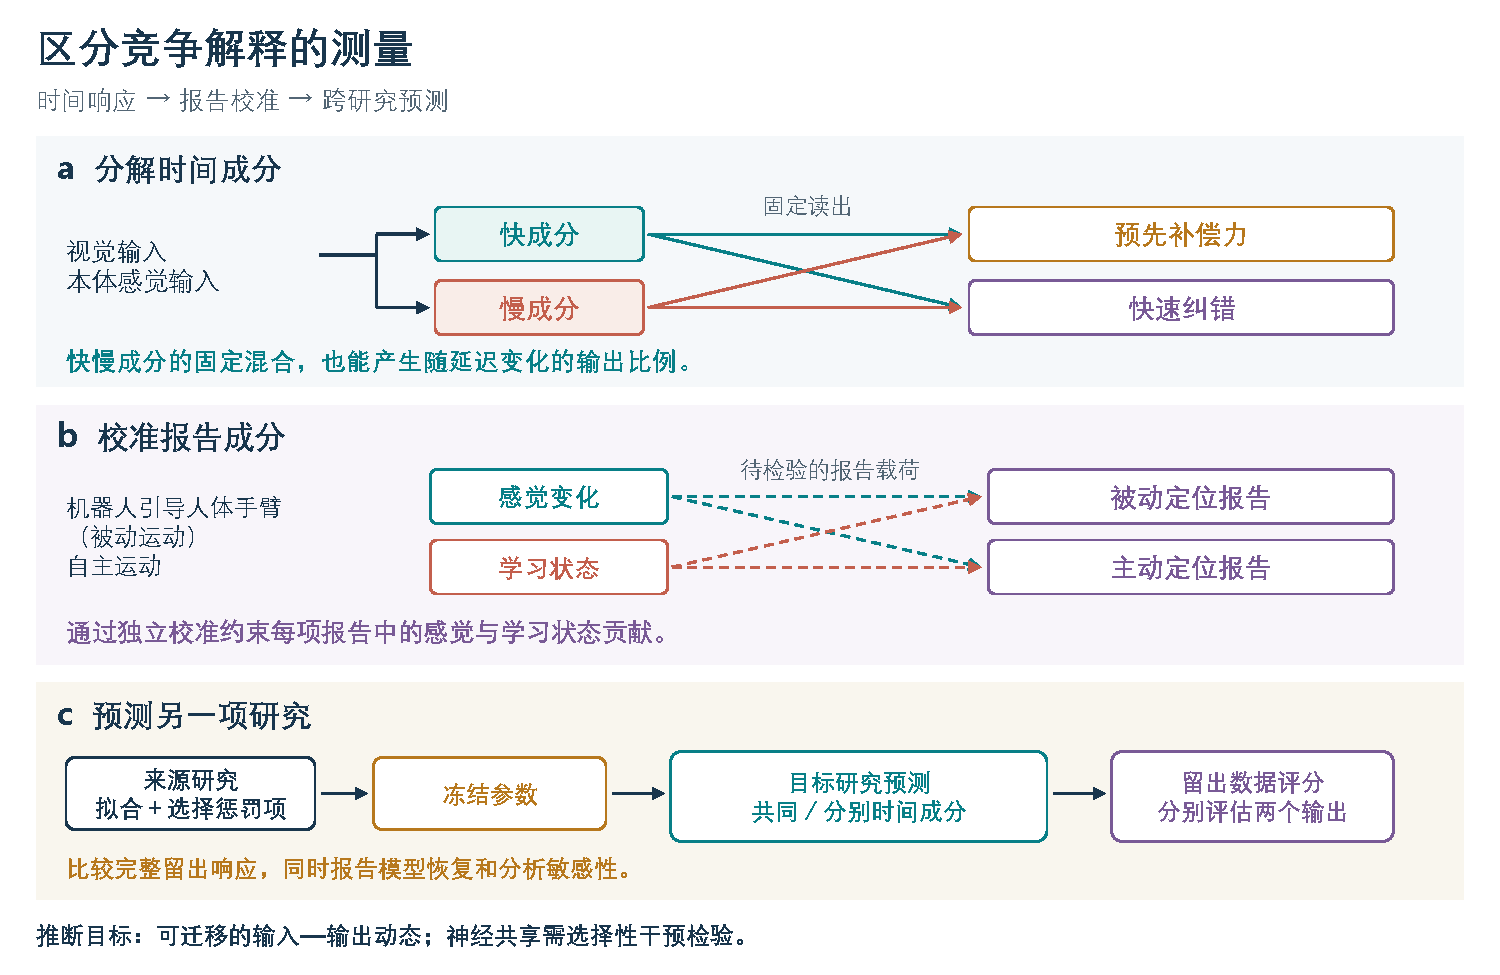
\includegraphics[width=\textwidth]{figure2_zh.pdf}
\caption{检验时间混合、报告载荷及外部预测。固定混合读出能够改变延迟比例；实线连接时间成分与两项测量输出；虚线表示定位报告的候选贡献，报告载荷由独立校准约束。被动运动指机器人引导人体手臂运动。来源拟合参数在目标研究评分前冻结。本图由PowerPoint原生对象组成。}
\end{figure}
\FloatBarrier
\small\begin{longtable}{p{.20\textwidth}p{.34\textwidth}p{.36\textwidth}}
\caption{由证据导出的追加测量选择；完整对照与模拟边界见图谱。}\label{tab:rules}\\\toprule
争议 & 最小追加测量 & 结果解释\\\midrule\endfirsthead\toprule
争议 & 最小追加测量 & 结果解释\\\midrule\endhead\bottomrule\endfoot
R1 共享更新与情境依赖表达 & 交叉训练与测试线索；在新误差出现前读取首次探针。 & 测试线索效应识别表达；共同测试线索下保留的训练效应推动更新/保持比较。\\[9pt]
R2 输入变化与混合报告载荷下的更新 & 增加主动/被动报告及独立载荷校准，在新情境检验报告预测。 & 预测分离支持因子对比；未知或共线载荷保留连续等价分解。\\[9pt]
R3 固定时间复制与整合教学信号 & 增加两个误差起始时点及晚期反转；记录完整纠错、保持与下一试次波形。 & 时间位移支持复制；学习时间保持而持续幅度可预测学习，支持整合。\\[9pt]
R4 神经增益与阻抗 & 增加背景肌电及小幅多方向机械扰动，并按潜伏期分解。 & 刚度变化解释力学贡献；匹配力学后的残余响应结构约束神经控制。\\[9pt]
R5 获得差异与保持或探针诱发学习差异 & 在多个延迟使用独立首次探针；平衡通道中的视觉反馈。 & 早期差异支持获得/读出效应；晚期分歧指向保持与探针暴露。\\[9pt]
R6 混合读出的共同时间模式与输出特异模式 & 在多个独立延迟测量两个输出，并留出新延迟或历史。 & 比例变化排除有效单模式轨迹；共同递推检验共同时间动力学。\\[9pt]
R7 机制共享与统计稳定化 & 匹配有效正则化，充分优化所有竞争模型，跨真实噪声与近等价实例评估恢复。 & 预测优势确立预测效用；机制选择还需要可区分干预预测及可靠恢复。\\[9pt]
R8 任务误差交互与策略叠加、注意调节 & 交叉任务误差、固定光标误差、目标闪烁及指示，采集匹配瞄准报告与即时无反馈后效。 & 控制瞄准与注意后的残余任务误差斜率支持交互；改善对指示敏感而隐式后效稳定，支持策略叠加。\\[9pt]
\end{longtable}\normalsize
\section{公开人体研究之间的冻结参数预测}
我们用两项公开力场研究检验时间响应的跨研究迁移：适应中保留或移除视觉误差信息，每项研究12人。两项均包含突然及渐变力场、通道补偿与视觉诱发力。我们重建存档块级观测，依次用完整一项研究训练并预测另一项。正则化由来源研究的参与者交叉验证选择；目标评分前冻结全部动力学参数及输出系数。目标暴露前均值用于基线校准，同时报告完全沿用来源基线的敏感性分析。主要响应窗为180--230 ms，另行报告230--300 ms。两种条件来自不同队列，迁移同时检验研究变化及感觉变化。\cite{franklin2021,franklin2023}

四个候选分别为单共同模式（三参数）、每输出单模式（四参数）、混合读出的双共同模式（六参数）及每输出双模式（八参数）。块级方程为$z_{r,t+1}=p_rz_{r,t}+(1-p_r)f_t$及$y_{i,t}=\sum_r c_{ir}(z_{r,t}+z_{r,t+1})/2$。全部候选使用相同力场序列、初始状态、稳定极点范围、观测时序及来源数据输出尺度。极点表示有效闭环块级持续性，其神经保持与误差敏感性因子未被分别测量。接近的双极点采用差商基底及其导数极限，避免巨大正负系数抵消。给定极点时精确求解线性系数；最终拟合采用64个初值。正则强度通过来源参与者六折验证从相同五值中选择，同时保留无正则预测。暴露前基线与来源研究的阶段均值模板提供简单比较对象。

主要时间窗中，增加第二共同模式使标准化预测MSE在视觉误差研究预测视觉钳制研究时改变-0.850 [-1.296, -0.472]，反方向改变-0.459 [-0.627, -0.292]。双分别模式减双共同模式的差异依次为-0.040 [-0.075, -0.002]及-0.009 [-0.027, 0.008]。括号为固定已训练来源模型、按目标参与者配对自助法得到的95\%区间。从视觉误差研究预测视觉钳制研究时，正则比较在主要时间窗支持分别模式，第二时间窗方向反转，无正则比较则跨越零；反方向研究的主要时间窗差异也跨越零。因此，架构排序依赖观测时间窗及正则设定。时间复杂性带来的联合改善主要集中于补偿；反馈力RMSE约为1.8--2.0 N，阶段模板在该输出上也具有竞争力。因此，实测预测收益涉及时间响应的丰富性，这一比较对共享与分别模式的分辨较弱。图谱附完整分输出评分、第二时间窗、基线迁移及无正则拟合。

新增实例恢复使用来源拟合家族、扰动后的参数及人体残差轨迹的配对五块重采样。每个合成组平均十二份参与者残差抽样，保留双通道配对及短时依赖。候选拟合突然暴露并预测渐变暴露。80个实例（每家族20个，平衡机会参照25\%）的强制家族分类恢复率为51.2\%。混淆矩阵完整报告，近等价预测不被转换为共享存储结论。共同模式的输出特异副本在任何噪声或优化精度下均保持观测等价。这一恢复实验测量该方案中有效时间核家族的实际可分性。


\begin{figure}[!htbp]\centering
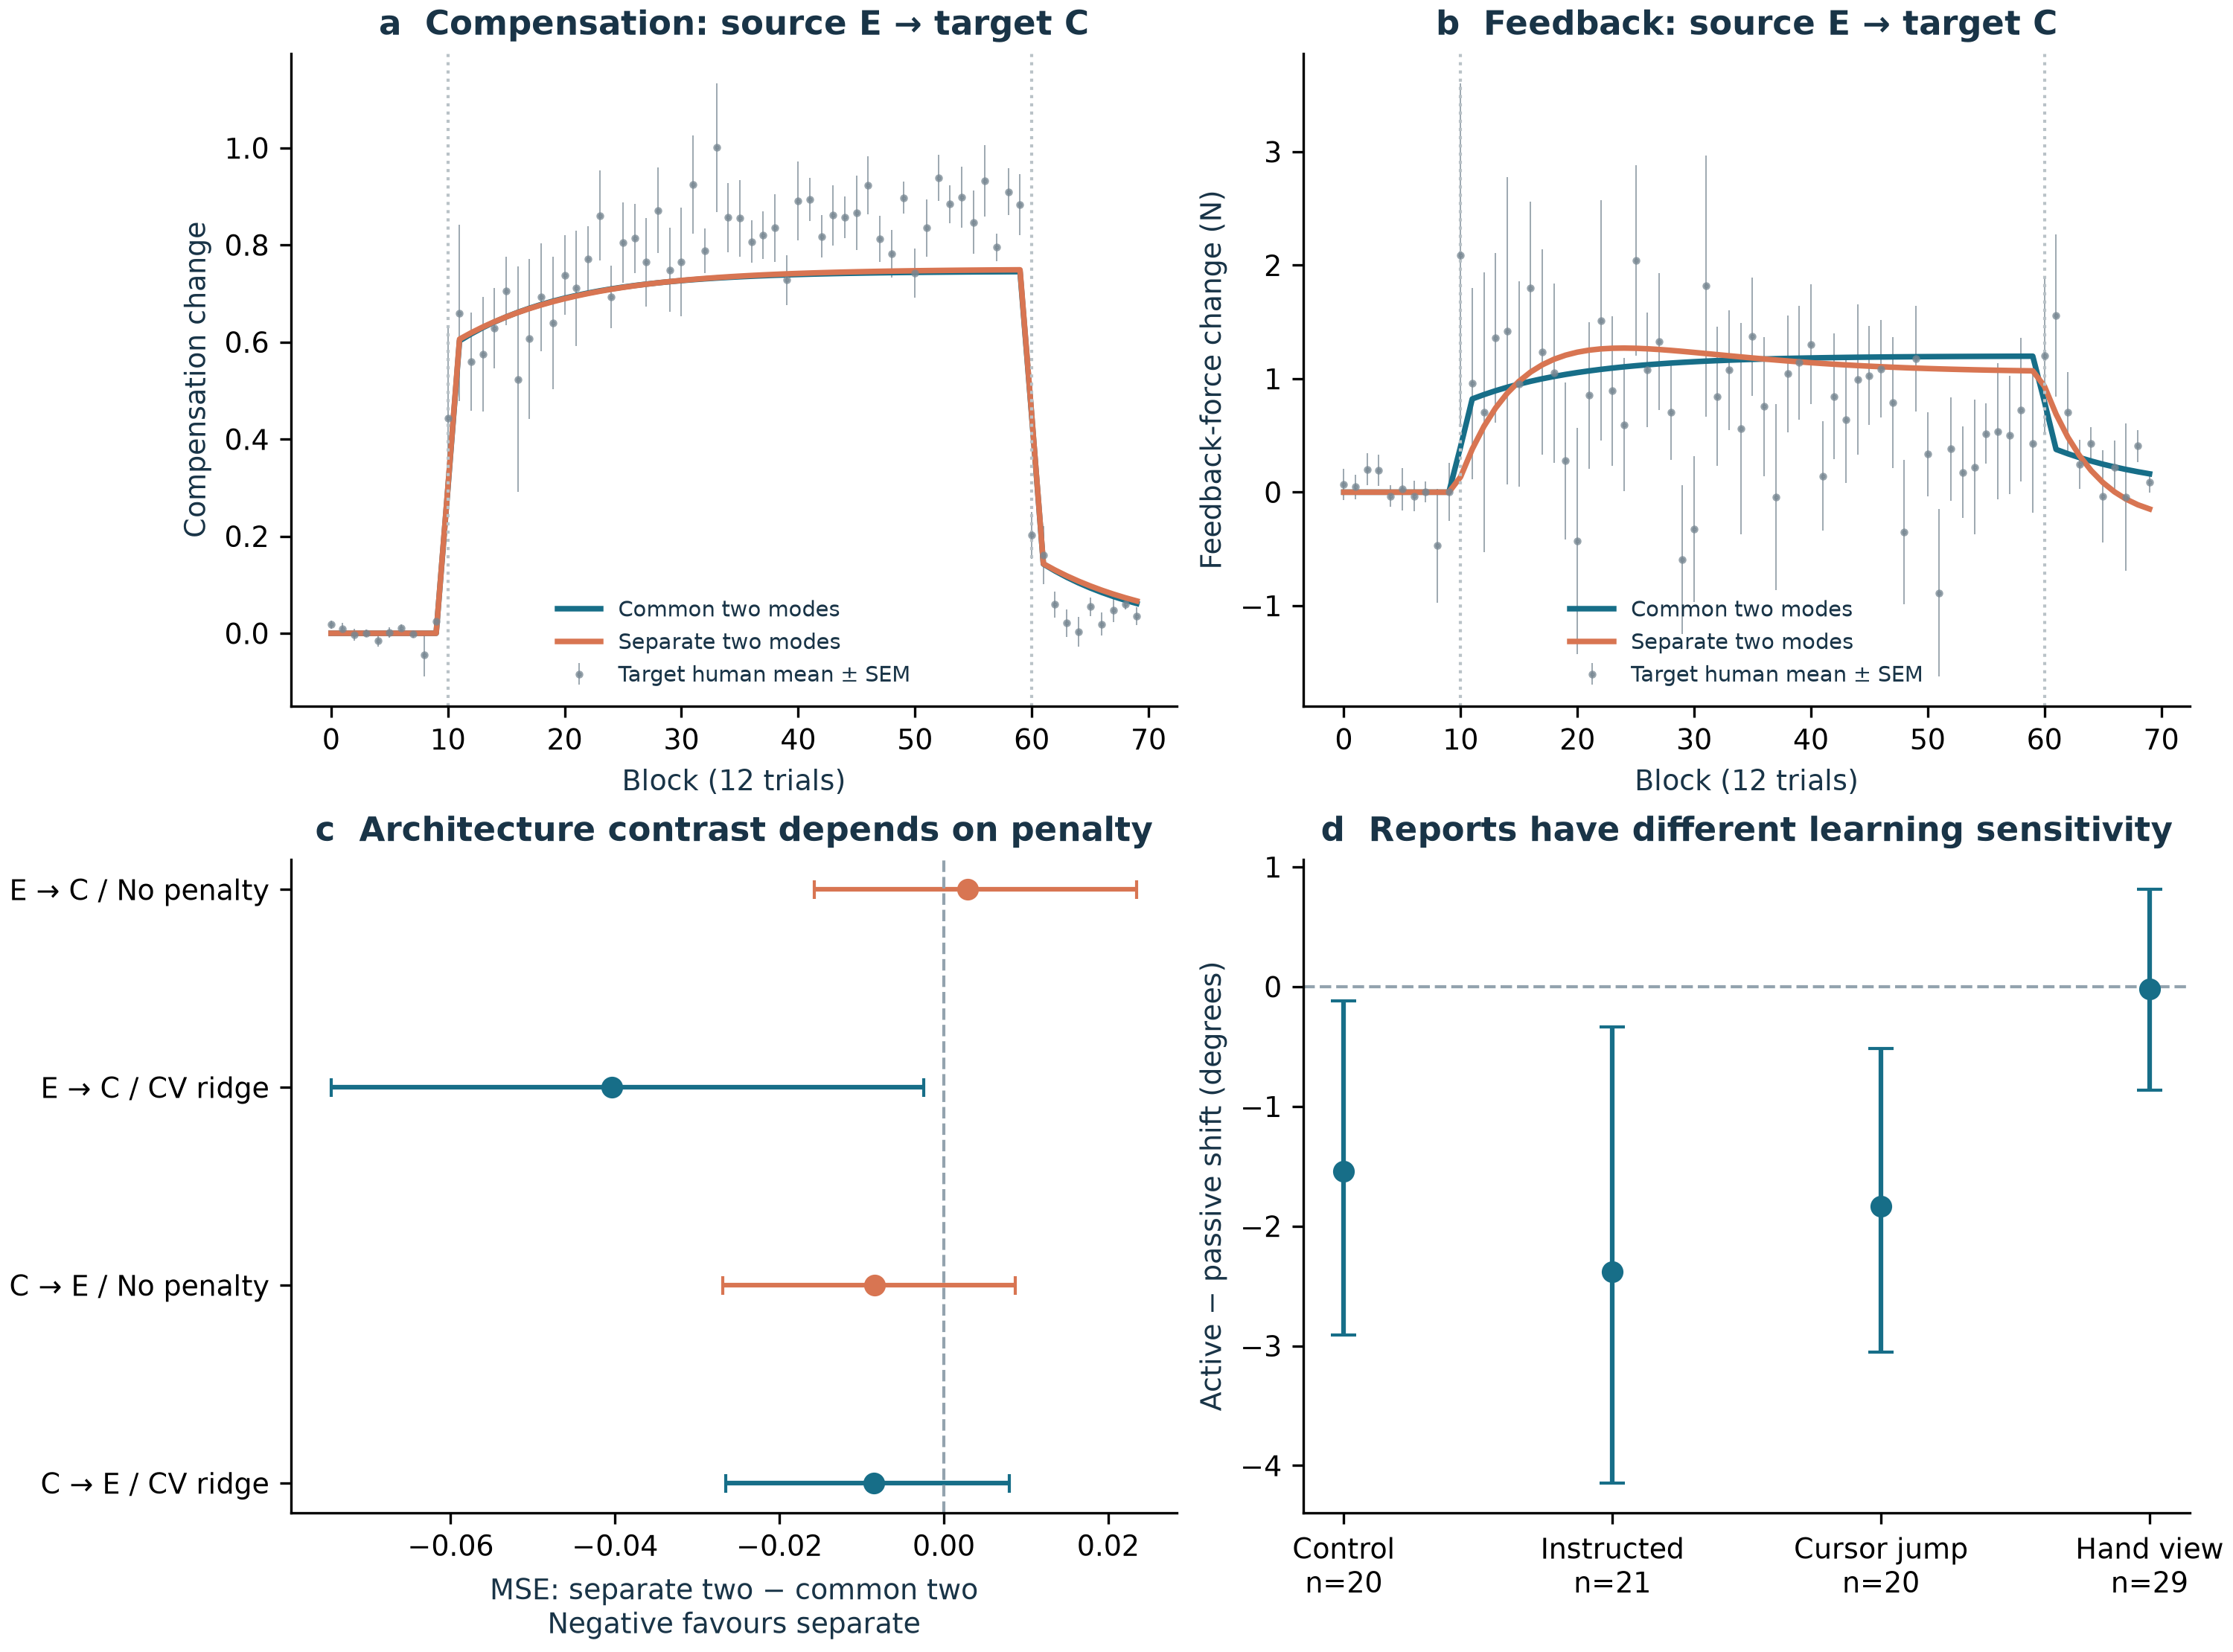
\includegraphics[width=\textwidth]{empirical_validation.png}
\caption{公开数据预测与校准检查。a、b：突然暴露中目标研究均值变化（点及参与者SEM）与冻结来源预测；附完整序列评分。c：双分别减双共同模式的联合标准化MSE配对差异及目标参与者自助法95\%区间。d：主动减被动定位变化及参与者自助法95\%区间。点与曲线由公开人体数据计算，未使用图像生成。}
\end{figure}
\section{哪些结果能够推进解释}
三个预测组织下一步实验。第一，\emph{条件性迁移}：若来源证据改变有效学习分配，那么在共同测试情境中，校准后的迁移矩阵应保留来源乘误差通道交互。若差异只随测试线索变化，结果支持情境依赖表达；若独立验证的报告载荷通过输入变化解释效应，该解释应预测联合留出响应。第二，\emph{时间选择性}：复制解释与整合教学解释应在留出的误差起始时点和符号反转试次上产生分歧。第三，\emph{正交维度上的共享}：不同感觉学习动态可以与向预先准备及纠错两个输出的迁移并存；观察到这一组合将支持结构化的多输入架构。

这些预测建立在已有贡献上。来源推断已用于解释泛化，情境推断已区分更新与表达，反馈—学习比较已检验教学信号，感觉特异学习已挑战标量误差解释。本文的贡献是将它们连接成统一的证据—实验映射，明确何种追加测量会改变推断结论。最有信息量的结果，是在相应机制所需对照下保持稳定、可重复的模式，同时保留与该模式兼容的神经实现。\cite{berniker2008,coin2021,albert2016,hayashi2020}

机器人操作为这一逻辑提供干预测试平台。在拟议微装配实验中，可以分别改变相机校准、接触力学或控制器记忆，将控制器训练至匹配的放置精度，再检验配对探针能否正确识别被操纵的成分。基于视觉的放置测量应配以接触力和释放测量，留出零件或表面用于测试迁移。这是一项拟议测量程序验证；生物学迁移需要具有对应感觉与控制测量的人体数据。共同价值在于可以直接干预原本混杂的因素。

由此形成的图景是：有用知识分布于感觉表征、适应状态与情境敏感输出之间。迁移和分离揭示这些成分如何相互作用，而对联合后果的测量将这一图景转化为逐步推进的判别实验。

\section{透明性与可复核材料}
随附配对证据、冻结预测、参与者评分、模型拟合、精确反例及可执行脚本。公开数据分析为所引研究的二次分析；目标暴露后观测未用于拟合及正则选择。分析在先前查阅广泛档案后开发，属于回顾性研究。恢复检验使用新抽取合成实例。图1--2通过AI辅助布局代码在Microsoft PowerPoint中重建为可编辑文字与矢量图形；早期草稿使用过OpenAI生成的概念图。当前图中不含生成图像像素。定量图直接由分析输出生成。语言模型辅助用于文献组织、双语撰写及代码准备。
\section{数据可用性}
本研究二次分析Franklin与Franklin（2021、2023）及Gastrock等（2020）的公开人体数据。来源记录和数据集标识符见随附public\_data元数据。处理后的块级观测、参与者定位估计、模型预测及分析摘要包含于随附复现材料包。\cite{franklin2021,franklin2023,external2020}
\section{代码可用性}
代码与复现材料见\href{https://github.com/WUJIAHAO-HKU/Shared-and-separable-motor-learning-reconciling-transfer-dissociation-and-error-attribution}{项目仓库}。材料包提供用于数据提取核查、时间模型拟合、跨研究预测、模型恢复、校准案例及定量图的Python脚本。README说明运行流程与依赖，发布清单记录文件哈希。
\section{作者贡献}
JiaHao Wu负责构思、文献整理、分析、代码开发及论文写作。曾龙提供指导。
\section{利益冲突}
作者声明不存在利益冲突。
\section{资助}
本工作未获得专项资助。

\begingroup\fontsize{8.5}{9.6}\selectfont\setlength{\parskip}{0pt}\setlength{\bibsep}{1pt}\bibliographystyle{unsrtnat}\bibliography{references}\endgroup\end{document}